\section{Theorie}
\label{sec:Theorie}

\subsection{Der Glühelektrische Effekt}
Ein Metall kann meist wie ein kristalliner Festkörper betrachtet werden.
Die ionisierten Leitungselektronen können sich im Inneren des Metalls recht frei
bewegen, da sie sich im Kraftfeld aller Ionen statt dem Kraftfeld eines Atoms
befinden. Ihre Beweglichkeit ähnelt den Molekülen innerhalb eines Gases.
Das Potential in dem sich die Leitungselektronen bewegen, kann in grober
Näherung als konstant betrachtet werden. Es unterscheidet sich von dem Potential
außerhalb des Metalls um den Betrag $\Phi$.
Um das Metall verlassen zu können, muss daher gegen ein Potential $\xi$ angelaufen
werden. Daraus ergibt sich eine zu leistende Austrittsarbeit von $e_0 \xi$,
wobei $e_0$ die Elementarladung bezeichnet.
Dieser Sachverhalt lässt sich gut mit einem Potentialtopf-Modell illustrieren:
\begin{figure}[H]
  \centering
  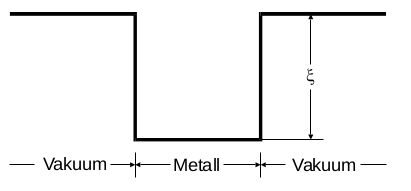
\includegraphics[scale=0.5]{content/potentialtopf.png}
  \caption{Potentialtopf-Modell eines Metalls.}
  \label{fig:potentialtopf}
\end{figure}
\noindent
Nach der Quantentheorie können die Elektronen nur diskrete Werte besitzen, welche
jedoch sehr nahe beieinanderliegen. Nach dem Pauli-Verbot kann jeder
mögliche Energiezustand nur von maximal zwei Elektronen mit entgegengestztem Spin
angenommen werden. Daher besitzen die Elektronen auch am absoluten Energienullpunkt
noch eine endliche Energie. Die Wahrscheinlichkeit, das ein Elektron eine bestimmte
Energie $E$ annimmt, wird durch die Fermi-Diracsche Verteilungsfunktion angegeben:
\begin{equation}
  f(E) = \frac{1}{e^{\frac{E - \xi}{k T}} + 1}.
  \label{eqn:fermidirac}
\end{equation}
\noindent
Hierbei bezeichnet $\xi$ die Fermische Grenzenergie, welche die Maximalenergie
der Elektronen bei $T = 0$ in Abhängigkeit der Zahl $n$ der Elektronen pro
Volumeneinheit des Metalls angibt. Bei Zimmertemperatur gilt für die Fermische
Grenzenergie $\xi >> kT$. Der Verlauf der Fermi-Dirac Verteilung ist folgender
Abbildung zu entnehmen:
\begin{figure}[H]
  \centering
  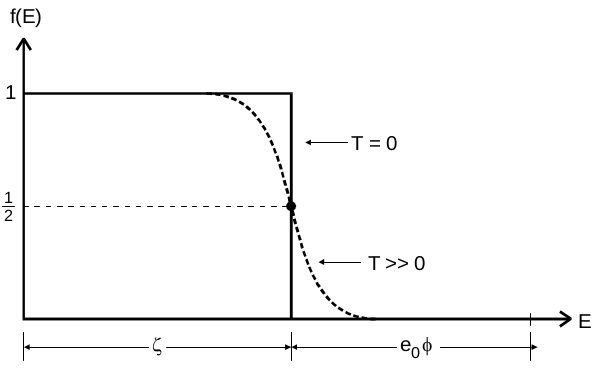
\includegraphics[scale=0.5]{content/fermidirac.png}
  \caption{Verlauf der Fermi-Dirac Verteilung.}
  \label{fig:fermidirac}
\end{figure}
\noindent
Ein Elektron benötigt daher zum Verlassen des Metalls eine Energie von
$\xi + e_0 \Phi$. Für diesen Wert gilt auch am Schmelzpunkt des Wolframs
$\xi + e_0 \Phi >> kT$. Aus diesem Grund kann man für die Elektronen, welche
das Metall verlassen, die Gleichung \eqref{eqn:fermidirac} durch Folgende nähern:
\begin{equation}
  \centering
  f(E) \approx e^{\frac{\xi -E}{kt}}.
  \label{eqn:approxfermidirac}
\end{equation}
\noindent

\subsection{Die Sättigungsstromdichte}
Die Sättigungsstromdichte beschreibt die Anzahl der Elektronen, die pro Zeiteinheit
und Flächeneinheit aus der Metalloberfläche heraustreten in Abhängigkeit von
der Temperatur. Hierfür wird ein Koordinatensystem mit Z-Achse orthogonal zu der
Metalloberfläche eingeführt. Mithilfe von Gleichung \eqref{eqn:approxfermidirac}
sowie der Anzahl $d\alpha$ der Elektronen aus dem Volumenelement des Impulsraumes
kann man zeigen, das folgendes gilt:
\begin{equation}
    d\alpha = \frac{\partial E}{\partial p_z} n(E) dp_x dp_y
    dp_z = n(E) dE dp_x dp_y dp_z.
    \label{eqn:elektronenvolumenelement}
\end{equation}
Hierbei beschreibt $n(E)$ die Zahl der Elektronen pro Volumeneinheit ihres
Phasenraumes. Hier kann verwendet werden, dass jeder Quantenzustand im Phasenraum
das Volumen $h^3$ einnimmt, woraus folgt:
\begin{equation}
    n(E) = \frac{2}{h^3}f(E).
    \label{eqn:anzahlelektronen}
\end{equation}
Hierbei beschreibt $f(E)$ die Wahrscheinlichkeit, mit der ein zur Energie $E$
gehörendes Element des Phasenraumes besetzt ist.
Aus Gleichung \eqref{eqn:elektronenvolumenelement} und \eqref{eqn:anzahlelektronen}
ergibt sich, dass nur die Elektronen die Metalloberfläche verlassen können, für
die gilt:
\begin{equation}
    \frac{p_z^2}{2 m_0} > \xi + e_0 \Phi.
    \label{eqn:elektronengeschwkomponente}
\end{equation}
Die Sättigungsstromdichte ergibt sich nun durch Abzählen aller Elektronen,
deren Geschwindigkeitskomponente in $z$-Richtung Gleichung
\eqref{eqn:elektronengeschwkomponente} erfüllen. Dieser Wert muss dann mit $e_0$
multipliziert werden. Hierraus ergibt sich die Richardson-Gleichung:
\begin{equation}
    j_s(T) = 4 \pi \frac{e_0 m_0 k^2}{h^3}T^2 \text{exp}\left(\frac{-e_0 \Phi}{k T}\right).
    \label{eqn:richardson}
\end{equation}

\subsection{Die Hochvakuum-Diode}
